\chapter{Entwurf}
\thispagestyle{standard}
\pagestyle{standard}
\renewcommand{\footrulewidth}{0.4pt}
\lfoot{\small Refik Kerimi}

In diesem Kapitel wird das Adaptermuster im Allgemeinen und die Anforderungen bzw. die Umsetzung des \aclp{PA} betrachtet.
Wie in Kapitel \ref{CM} beschrieben, erhöhen die jeweiligen Protokolladapter die Flexibilität und die Erweiterungsmöglichkeiten des OpenNES Systems. 


\section{Übersicht Adapter Pattern}\label{sub:Übersicht Adapter Pattern}
In \upshape \cite{GOF} wird ein Adapter wie folgt definiert:
\begin{quote}
"Convert the interface of a class into another interface clients expect. \\Adapter lets classes work together that couldn't otherwise because of incompatible interfaces" (\cite{GOF} Seite 157).
  
  \end{quote}

\begin{figure}[h]
	\centering
	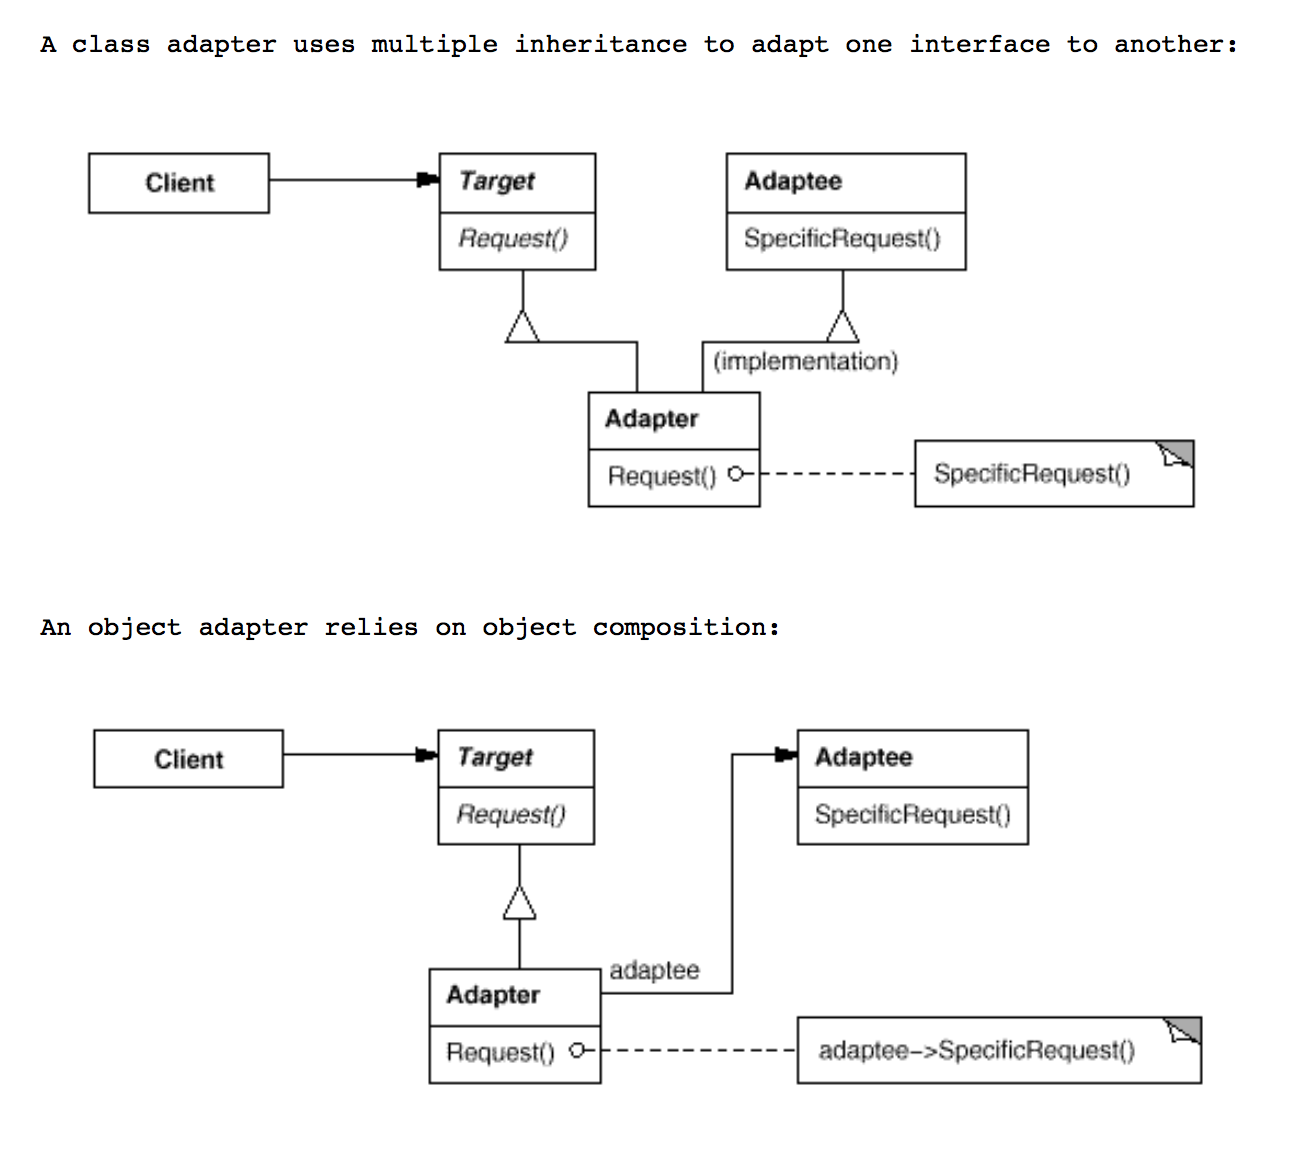
\includegraphics[width=14cm]{BilderAllgemein/O_K_Adapter}\medskip
 	\caption{UML Diagramm des Objekt- bzw. Klassenadapters \upshape \cite [ S.159]{GOF}}
 	\label{fig:Objekt- bzw. Klassenadapter}
\end{figure}

Wie in Abbildung \ref{fig:Objekt- bzw. Klassenadapter} dargestellt, gibt es zwei Möglichkeiten, die Adapter zu implementieren.
Klassen- und Objektadapter verwenden verschiedene Arten der Adaption.
Der Klassenadapter bildet eine Unterklasse des Adaptee und des Ziels, wohingegen der Objektadapter die Zielschnittstelle implementiert \cite{AdaptPattern, GOF}. 


Die Adapter Pattern werden wie in \upshape \cite{GOF} beschrieben verwendet: 
   \begin{itemize}
      \item wenn das Interface der bestehenden Klasse nicht zur benötigten Klasse passt
      \item wenn wiederverwendbare Klassen benötigt werden, die über keine kompatiblen Schnittstellen verfügen
      \item um Unterklassen in ein System zu implementieren, ohne die Schnittstellen der Unterklassen zu verändern
   \end{itemize}
Der OpenNES Protokolladapter entspricht vor allem dem letzten Punkt.
Wie in der Abbildung \ref{CM} zu sehen ist, verhält sich der Adapter als Unterklasse der jeweiligen Protokolle.
Dadurch können die Funktionscodes des Modbus Protokolls so genutzt werden, dass das geforderte Messaging Muster dabei erfüllt wird. 

\section{Anforderungsanalyse}\label{sub:Anforderungsanalyse}
Im Zuge der Bachelorarbeit werden folgende Anforderungen an den \ac{PA} gestellt.
Der \acs{PA} im OpenNES SmartOS soll Teil des übergeordneten Connectivity Moduls sein.
Da diverse Netzwerkstrukturen bereits vorhanden sind und unterschiedliche Protokolle wie IEC 61850, ModBus, XMPP, DNP3 etc. verwendet werden, soll der \acs{PA} ein Interface zu \acfp{IED} und \acp{SED} schaffen.
Als \acs{IED}s werden in diesem Kontext OpenNES fähige Geräte bezeichnet und als \acs{SED}s die Legacy Geräte.
Der Adapter soll dabei die Integration der Legacy Geräte ins OpenNES ermöglichen. 
Er soll eine Schnittstelle zur unteren Modbusschicht bieten und folgende Funktionen beinhalten:

\begin{itemize}
\item \textit{Push 1:1}  \\
Nachricht wird vom Sender zum Empfänger übertragen (siehe Kapitel \ref{sec:PushFunction}).

\item \textit{Push 1:N} \\
Bei der Push 1:n Funktion schreibt ein Client den Wert eines Datenpunktes auf eine Anzahl
von n Server (siehe Kapitel \ref{sec:RequRespFunction}).

\newpage
\item \textit{Request-Response} \\
Request Response besteht aus 2 Teilnehmern, Sender und Empfänger.
Diese Funktion fragt bestimmte Datenpunkte in Registern ab (z.B.: Holding Register) (siehe Kapitel \ref{sec:RequRespFunction}).


\item \textit{Publish-Subscribe} \\
Publish-Subscribe ist auch als Observer Pattern bekannt. 
Bei diesem Pattern sendet der Protokolladapter (Client) Anfragen an den Modbus Server und überprüft dabei, ob sich im Server Register Daten verändert wurden (siehe Kapitel \ref{sec:PublishSubscribeFunction}).

\end{itemize}

Weiters soll das Adressmapping zwischen der OpenNES Adressierung und der Adressierung der Adapter wie in Abbildung \ref{fig:SyntaxAMapping} umgesetzt werden.

\begin{figure}[h]
	\centering
	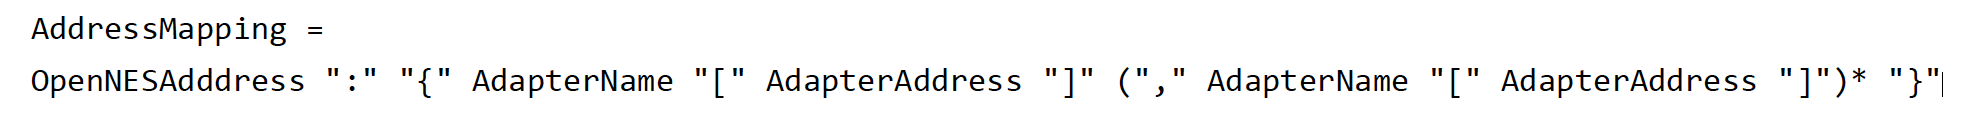
\includegraphics[width=16cm]{BilderAllgemein/SyntaxAMapping}\medskip
 	\caption{Adressmapping OpenNES zu Adapter}
 	\label{fig:SyntaxAMapping}
\end{figure}

Es bestehen mehrere Protokollstandards, wie in Punkt \ref{sub:Anforderungsanalyse} beschrieben wurde. 
Für dieses Projekt soll das  \textit{ModbusTCP/Sunspec Protokoll} verwendet werden.\\ Da der ModbusTCP keine Datenpunkte abbildet, wird der SunSpec Standard verwendet. Weiters soll der Adapter die vom OpenNES an das Connectivity Modul übergebene Adresse des  Servers in die Remote-Adresse für den Modbus übersetzen.
Das Ziel ist es, dass ein \acs{IED} mit mehreren \acsp{SED} kommuniziert.
Die Befehle, von welchem \acsp{SED} Informationen benötigt werden bzw. Daten geschrieben werden, kommen seitens des \acs{CM}.

